\paragraph*{线性与非线性边值问题的非唯一性}

\PDEIndexMark{idx:boundary-value-eigenvalue-prototype}虽然唯一性通常是人们希望问题的解具有的一种性质 (这往往出于物理原因), 但在某些情形下, 多个解才是人们所期望的. 涉及多个解的一种常见数学问题是特征值问题. 读者当然应当熟悉有限维线性代数中的各种存在性和多解性结果, 不过, 这里我们来考察几个常微分方程问题. 考虑下列依赖于参数 $\lambda$ 的二阶常微分方程:
\begin{equation}\label{eq:linear-mixed-boundary-ode}
u''+\lambda u=0.
\end{equation}

当然, 如果施加两个初始条件 (在空间中的同一个点处), 那么由 Theorem~\ref{thm:ode-uniqueness} 可知, 我们将得到唯一解. (要直接应用该定理, 需要把二阶方程问题转化为一阶方程组.) 然而, 如果施加两点边界条件
\begin{equation}\label{eq:linear-mixed-dirichlet}
u(0)=0,
\end{equation}
\begin{equation}\label{eq:linear-mixed-neumann}
u'(1)=0,
\end{equation}
上述唯一性定理就不再适用. 取而代之的是下面的结果.

\begin{Theorem}
\label{thm:linear-mixed-boundary-alternatives}
边值问题 \eqref{eq:linear-mixed-boundary-ode}, \eqref{eq:linear-mixed-dirichlet}, \eqref{eq:linear-mixed-neumann} 的解有以下两种情形.
\begin{enumerate}
\item 如果 $\lambda=\lambda_n:=((2n+1)^2\pi^2)/4$, $n=0,1,2,\ldots$, 那么该边值问题有一族以 $A\in(-\infty,\infty)$ 为参数的解:
\[
u_n(x)=A\sin\dfrac{(2n+1)\pi}{2}x.
\]
此时称 $\lambda$ 为特征值.
\item 对于 $\lambda$ 的所有其他取值, 该边值问题唯一的解是平凡解
\[
u(x)\equiv0.
\]
\end{enumerate}
\end{Theorem}

\PDEIndexMark{idx:nonlinear-beam-problem}或者具有唯一的 (平凡) 解, 或者具有一个无限的线性解族, 这是线性问题的典型特征. 对于非线性问题, 则有更有趣的多解性结果, 它们是现代\emph{分岔理论}的主要研究对象. 例如, 考虑下面的非线性边值问题, 它由 Euler 推导而来, 用以描述一根细长、均匀、不可伸长的竖直弹性梁在载荷 $\lambda$ 下的挠曲:
\begin{equation}\label{eq:euler-elastica}
\theta''(x)+\lambda\sin\theta(x)=0,
\end{equation}
\begin{equation}\label{eq:euler-elastica-dirichlet}
\theta(0)=0,
\end{equation}
\begin{equation}\label{eq:euler-elastica-neumann}
\theta'(1)=0.
\end{equation}

\begin{figure}[H]
\centering
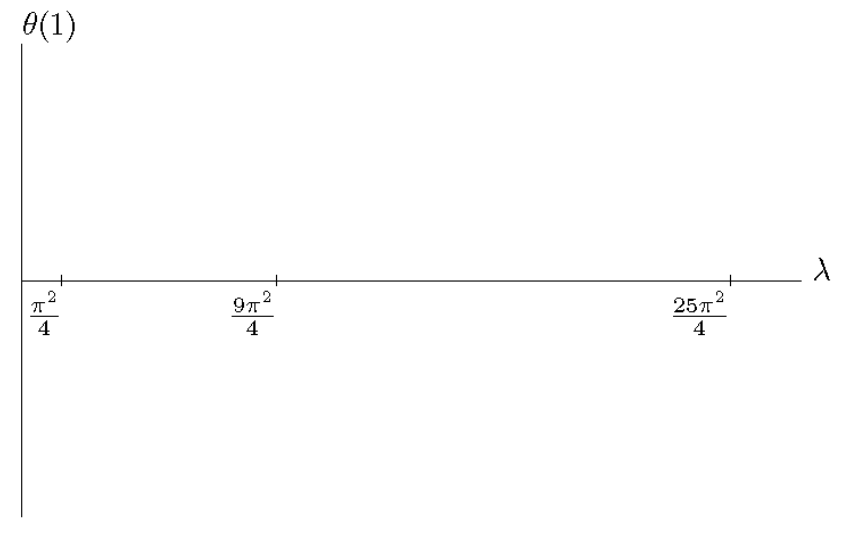
\includegraphics[width=.78\linewidth]{figures/beam-bifurcation-scan.png}
\caption{非线性边值问题的分岔图}\label{fig:beam-bifurcation}
\end{figure}

(注意, 当 $\theta$ 很小时, 线性常微分方程 \eqref{eq:linear-mixed-boundary-ode} 是 \eqref{eq:euler-elastica} 的近似.)

这一非线性边值问题的解已经用闭式形式计算出来 (用 Jacobi 椭圆函数表示), 而用 Figure~\ref{fig:beam-bifurcation} 这样的\emph{分岔图}来展示这些解, 可能最为合适. 该图把解 $\theta$ 的振幅表示为出现该解时 $\lambda$ 取值的函数. $\lambda$ 轴表示平凡解 $\theta\equiv0$ (它对每个 $\lambda$ 都成立). 注意, 非平凡解的一个\emph{分支}从上述线性问题的每个特征值处发出. 因此, 当 $\lambda\in(\lambda_{n-1},\lambda_n)$, $n=1,2,3,\ldots$ 时, 该边值问题恰好有 $2n$ 个非平凡解.

\subsubsection{稳定性}\label{subsec:stability}

稳定性一词在数学中具有多种不同的含义. 人们常说, 如果一个问题"关于数据连续", 那么它就是稳定的; 即如果将问题作"微小"改变时, 解也只发生微小改变, 就称该问题稳定. 下文将在常微分方程初值问题的背景下给出这一说法的精确定义. 另一种稳定性概念是"渐近稳定性". 这里, 如果当时间趋于无穷时, 一个问题的所有解都接近某个"良好"的解, 就称该问题稳定. 我们将通过一个关于常系数线性常微分方程组的结果, 使这一概念精确化.

\paragraph*{关于初始条件的稳定性}

本节假设 $\bm{F}$ 满足 Theorem~\ref{thm:ode-existence} 的假设, 并将 $\hat{\bm{y}}(t,t_0,\bm{y}_0)$ 定义为 \eqref{eq:ode-initial-value-dynamics}, \eqref{eq:ode-initial-value-data} 的唯一解. 于是有下面这个标准结果.

\begin{Theorem}{关于初始条件的连续性}
\label{thm:initial-data-continuity}
函数 $\hat{\bm{y}}$ 在一个开集上良定义:
\[
U\subset\mathbb{R}\times D.
\]
此外, 在每个 $(t,t_0,\bm{y}_0)\in U$ 处, 函数
\[
(t_0,\bm{y}_0)\mapsto\hat{\bm{y}}(t,t_0,\bm{y}_0)
\]
都是连续的; 即对于任意 $\epsilon>0$, 存在 $\delta$ (依赖于 $(t,t_0,\bm{y}_0)$ 和 $\epsilon$), 使得如果
\[
|(t_0,\bm{y}_0)-(\tilde{t}_0,\tilde{\bm{y}}_0)|<\delta,
\]
那么 $\hat{\bm{y}}(t,\tilde{t}_0,\tilde{\bm{y}}_0)$ 良定义, 且
\begin{equation}\label{eq:initial-data-continuity}
|\hat{\bm{y}}(t,t_0,\bm{y}_0)-\hat{\bm{y}}(t,\tilde{t}_0,\tilde{\bm{y}}_0)|<\epsilon.
\end{equation}
\end{Theorem}

因此可以看到, 初始条件的微小改变会引起初值问题的解的微小改变.
